\noindent \textred{2.} 
Build an AVL Tree out of the BST according to the rotation operations in the lecture with one rotation operation. The pre-order traversal sequence of the BST is \{10, 5, 3, 7, 6, 9, 8, 13, 11, 14\}. First \textbf{draw the BST}, then do the rotation. Also answer the type of this rotation (\textbf{Single} or \textbf{Double}). \\
\textblue{This is a single rotation.} \\
\begin{minipage}[t]{.4\textwidth}
    \vspace{0pt}
    \centering
    \includegraphics[width=\linewidth]{HWs//HW7//figures/2_1.png}
\end{minipage}
\hspace{30pt}
\begin{minipage}[t]{.5\textwidth}
    \vspace{0pt}
    \centering
    \includegraphics[width=\linewidth]{HWs//HW7//figures/2_2.png}
\end{minipage}

% \begin{figure}[!h]
%     \vspace{0pt}
%     \centering
%     \includegraphics[width=0.4\linewidth]{HWs/HW7/figures/2_1.png}
%     \qquad
%     \vspace{0pt}
%     \includegraphics[width=0.5\linewidth]{HWs/HW7/figures/2_2.png}
% \end{figure}